%\textsl{}%!TEX TS-options = --shell-escape
%!TEX TS-program = pdflatex
\documentclass[%
   10pt,              % Schriftgroesse
   nenglish,           % wird an andere Pakete weitergereicht
   a4paper,           % Seitengroesse
   DIV11,             % Textbereichsgroesse (siehe Koma Skript Dokumentation !)
]{scrartcl}%     Klassen: scrartcl, scrreprt, scrbook, article
% -------------------------------------------------------------------------

\usepackage[utf8]{inputenc} % Font Encoding, benoetigt fuer Umlaute
\usepackage[english]{babel}   % \textsl{}Spracheinstellung

\usepackage[T1]{fontenc} % T1 Schrift Encoding
\usepackage{textcomp}    % Zusatzliche Symbole (Text Companion font extension)
\usepackage{lmodern,dsfont}     % Latin Modern Schrift
\usepackage{dsfont}
%\usepackage{wasysym}
\usepackage{ulem}
\usepackage{graphicx}
\usepackage{grffile} %allows to use pngs
\usepackage{eurosym}
%\usepackage{txfonts}
\usepackage{stmaryrd}
\usepackage{amsfonts}
\usepackage{amsmath}
\usepackage{hyperref}
\usepackage{tikz}
\usepackage{multirow}
\usepackage{listings}
\usepackage{etextools}
\usepackage{ifthen}
\usepackage{TikZ} %phylogenetischer Baum
\usetikzlibrary{calc, shapes, backgrounds} %für die Phylogenetische bäume
\usetikzlibrary{automata,arrows}
\usepackage{subfigure} 


% Definition des Headers
\usepackage{geometry}
\geometry{a4paper, top=3cm, left=3cm, right=3cm, bottom=3cm, headsep=0mm, footskip=0mm}
\renewcommand{\baselinestretch}{1.3}\normalsize

\def\header#1#2#3#4#5#6#7{\pagestyle{empty}
\noindent
\begin{minipage}[t]{0.6\textwidth}
\begin{flushleft}
\textbf{#4}\\% Fach
#6\\% Semester
Tutor: #2  % Tutor 
\end{flushleft}
\end{minipage}
\begin{minipage}[t]{0.4\textwidth}
\begin{flushright}
\points{#7}% Punktetabelle
\vspace*{0.2cm}
#5%  Names
\end{flushright}
\end{minipage}

\begin{center}
{\Large\textbf{ Blatt #1}} % Blatt

{(Abgabe am #3)} % Abgabedatum
\end{center}
}

\newenvironment{vartab}[1]
{
    \begin{tabular}{ |c@{} *{#1}{c|} } %\hline
}{
    \end{tabular}
}

\newcommand{\myformat}[1]{& #1}

\newcommand{\entry}[1]{
  \edef\result{\csvloop[\myformat]{#1}}
  \result \\ \hline
}

\newcommand{\numbers}[1]{
  \newcounter{ctra}
\setcounter{ctra}{1}
\whiledo {\value{ctra} < #1}%
{%
  \myformat{\thectra}
  \stepcounter{ctra}%
}
\myformat{\thectra}
}
\newcommand{\emptyLine}[1]{
  \newcounter{ctra1}
\setcounter{ctra}{1}
\whiledo {\value{ctra1} < #1}%
{%
  \myformat{\hspace*{0.5cm}}
  \stepcounter{ctra1}%
}
}

\newcommand{\points}[1]{
\newcounter{colmns}
\setcounter{colmns}{#1}
\stepcounter{colmns}
  \begin{vartab}{\thecolmns}
    \numbers{#1} & $\sum$\\\hline
    \emptyLine{\thecolmns}\\
  \end{vartab}
}


\begin{document}
%\header{Blatt}{Tutor}{Abgabedatum}{Vorlesung}{Bearbeiter}{Semester}{Anzahl Aufgaben}
\header{7}{Alexander Seitz}{26. October 2015}{Bioinformatics I}{\\Jonas Ditz \\\& Benjamin Schroeder}{WS 15/16}{3}

 \section*{Exercise 1 - \textsl{Hirschberg algorithm for alignment in linear space}}
  With two given Sequences (X= TGGA and Y=TTGAGA), the scoring of s(a,a) = 4, s(a,b)=-3 and a gap penalty g=-3, the Hirschberg algorithm was started. First the sequence X was split into two substrings, one was the prefix (\ref{Step1}-green): TG and one the subfix sequence GGA (\ref{Step1} - yellow). The prefix was used in a NW alignment and the suffix was also used in a NW laigment, but this time reversed. Both NW Matrices were calculated with the space reduced algorithm technique. The result is an array with the maxima the matrix saved in an array (\ref{Step1}-red columns). Both arrays are cellwise added up and the maximum is used to determine the two positions of both sequences (\ref{Step1}-red cell), which should be aligned. In step 1 this was the G(X2) to the G(Y3). These position were finally saved in a final array.
 
 First, the Sequence X was split into two parts and 
  \begin{figure}[h]
  	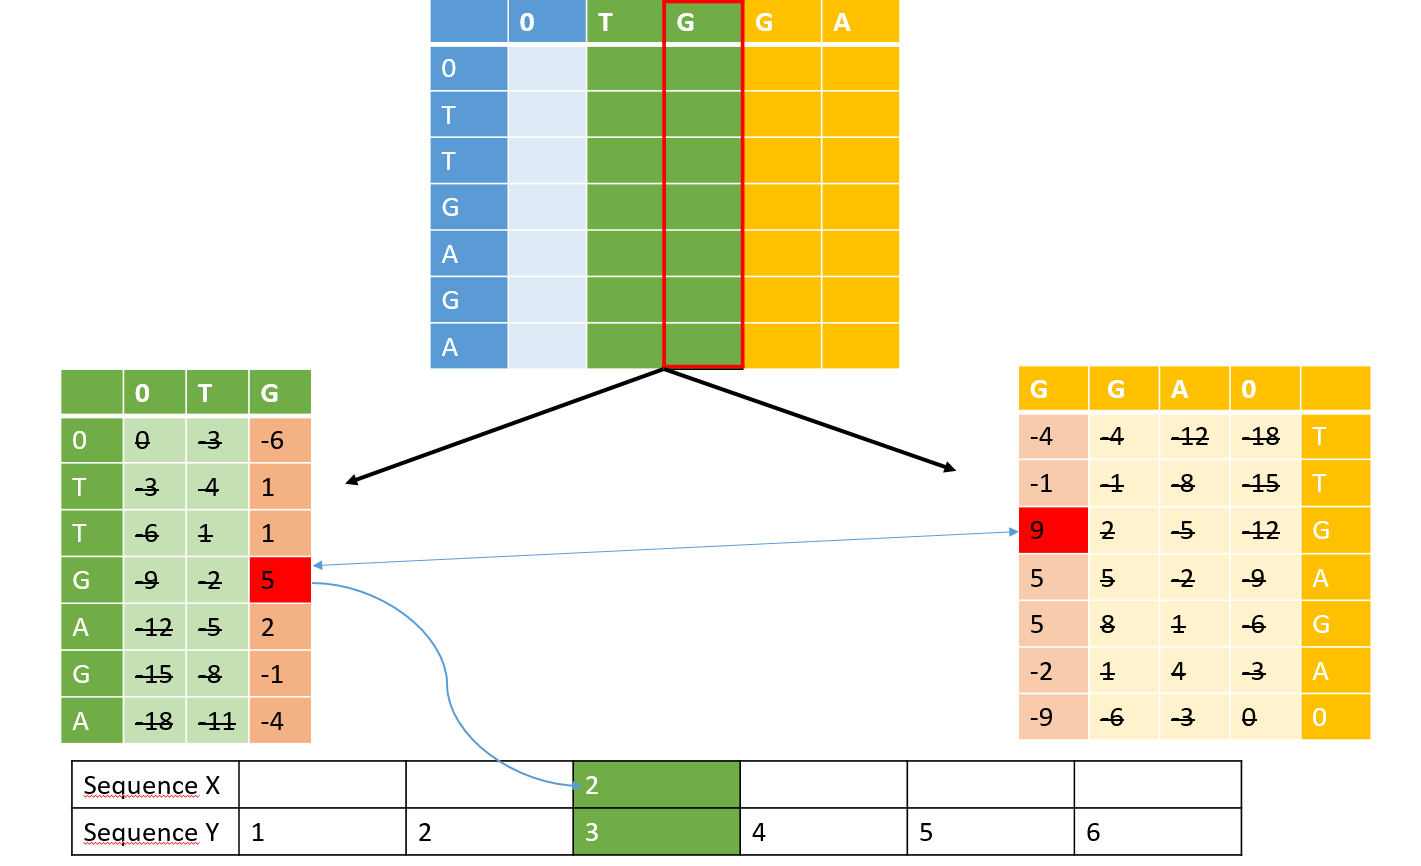
\includegraphics[scale=0.25]{img/Hirschberg_Step1.png}
  	\label{Step1}
  	\caption{In the first step the sequence X was split into two parts and for both a NW global alignment was calculated. It's important to state, that the NW of the suffix of the sequence splitting was calculated reverse. The Maximum which was found after the substraction of both maxima was used to identify two letters, whrch are to be aligned.}
  \end{figure}
  The second steps starts with cutting the  matrix in the Sequence Y Dimension. Definition of how to start the cutting is not very clearly described, and therefore we cutted at position y+1(\ref{Step2} - yellow and gold area) and y-1 (\ref{Step2} - green area) of the last maximum. The yellow and gold part was processed like in the first step. The green one was interpreted as the trivial case, were one sequence has the length one. which mean,s we simply took the maximum of the table as the to aligning position and saved it in the result array.
   
  \begin{figure}[h]
   	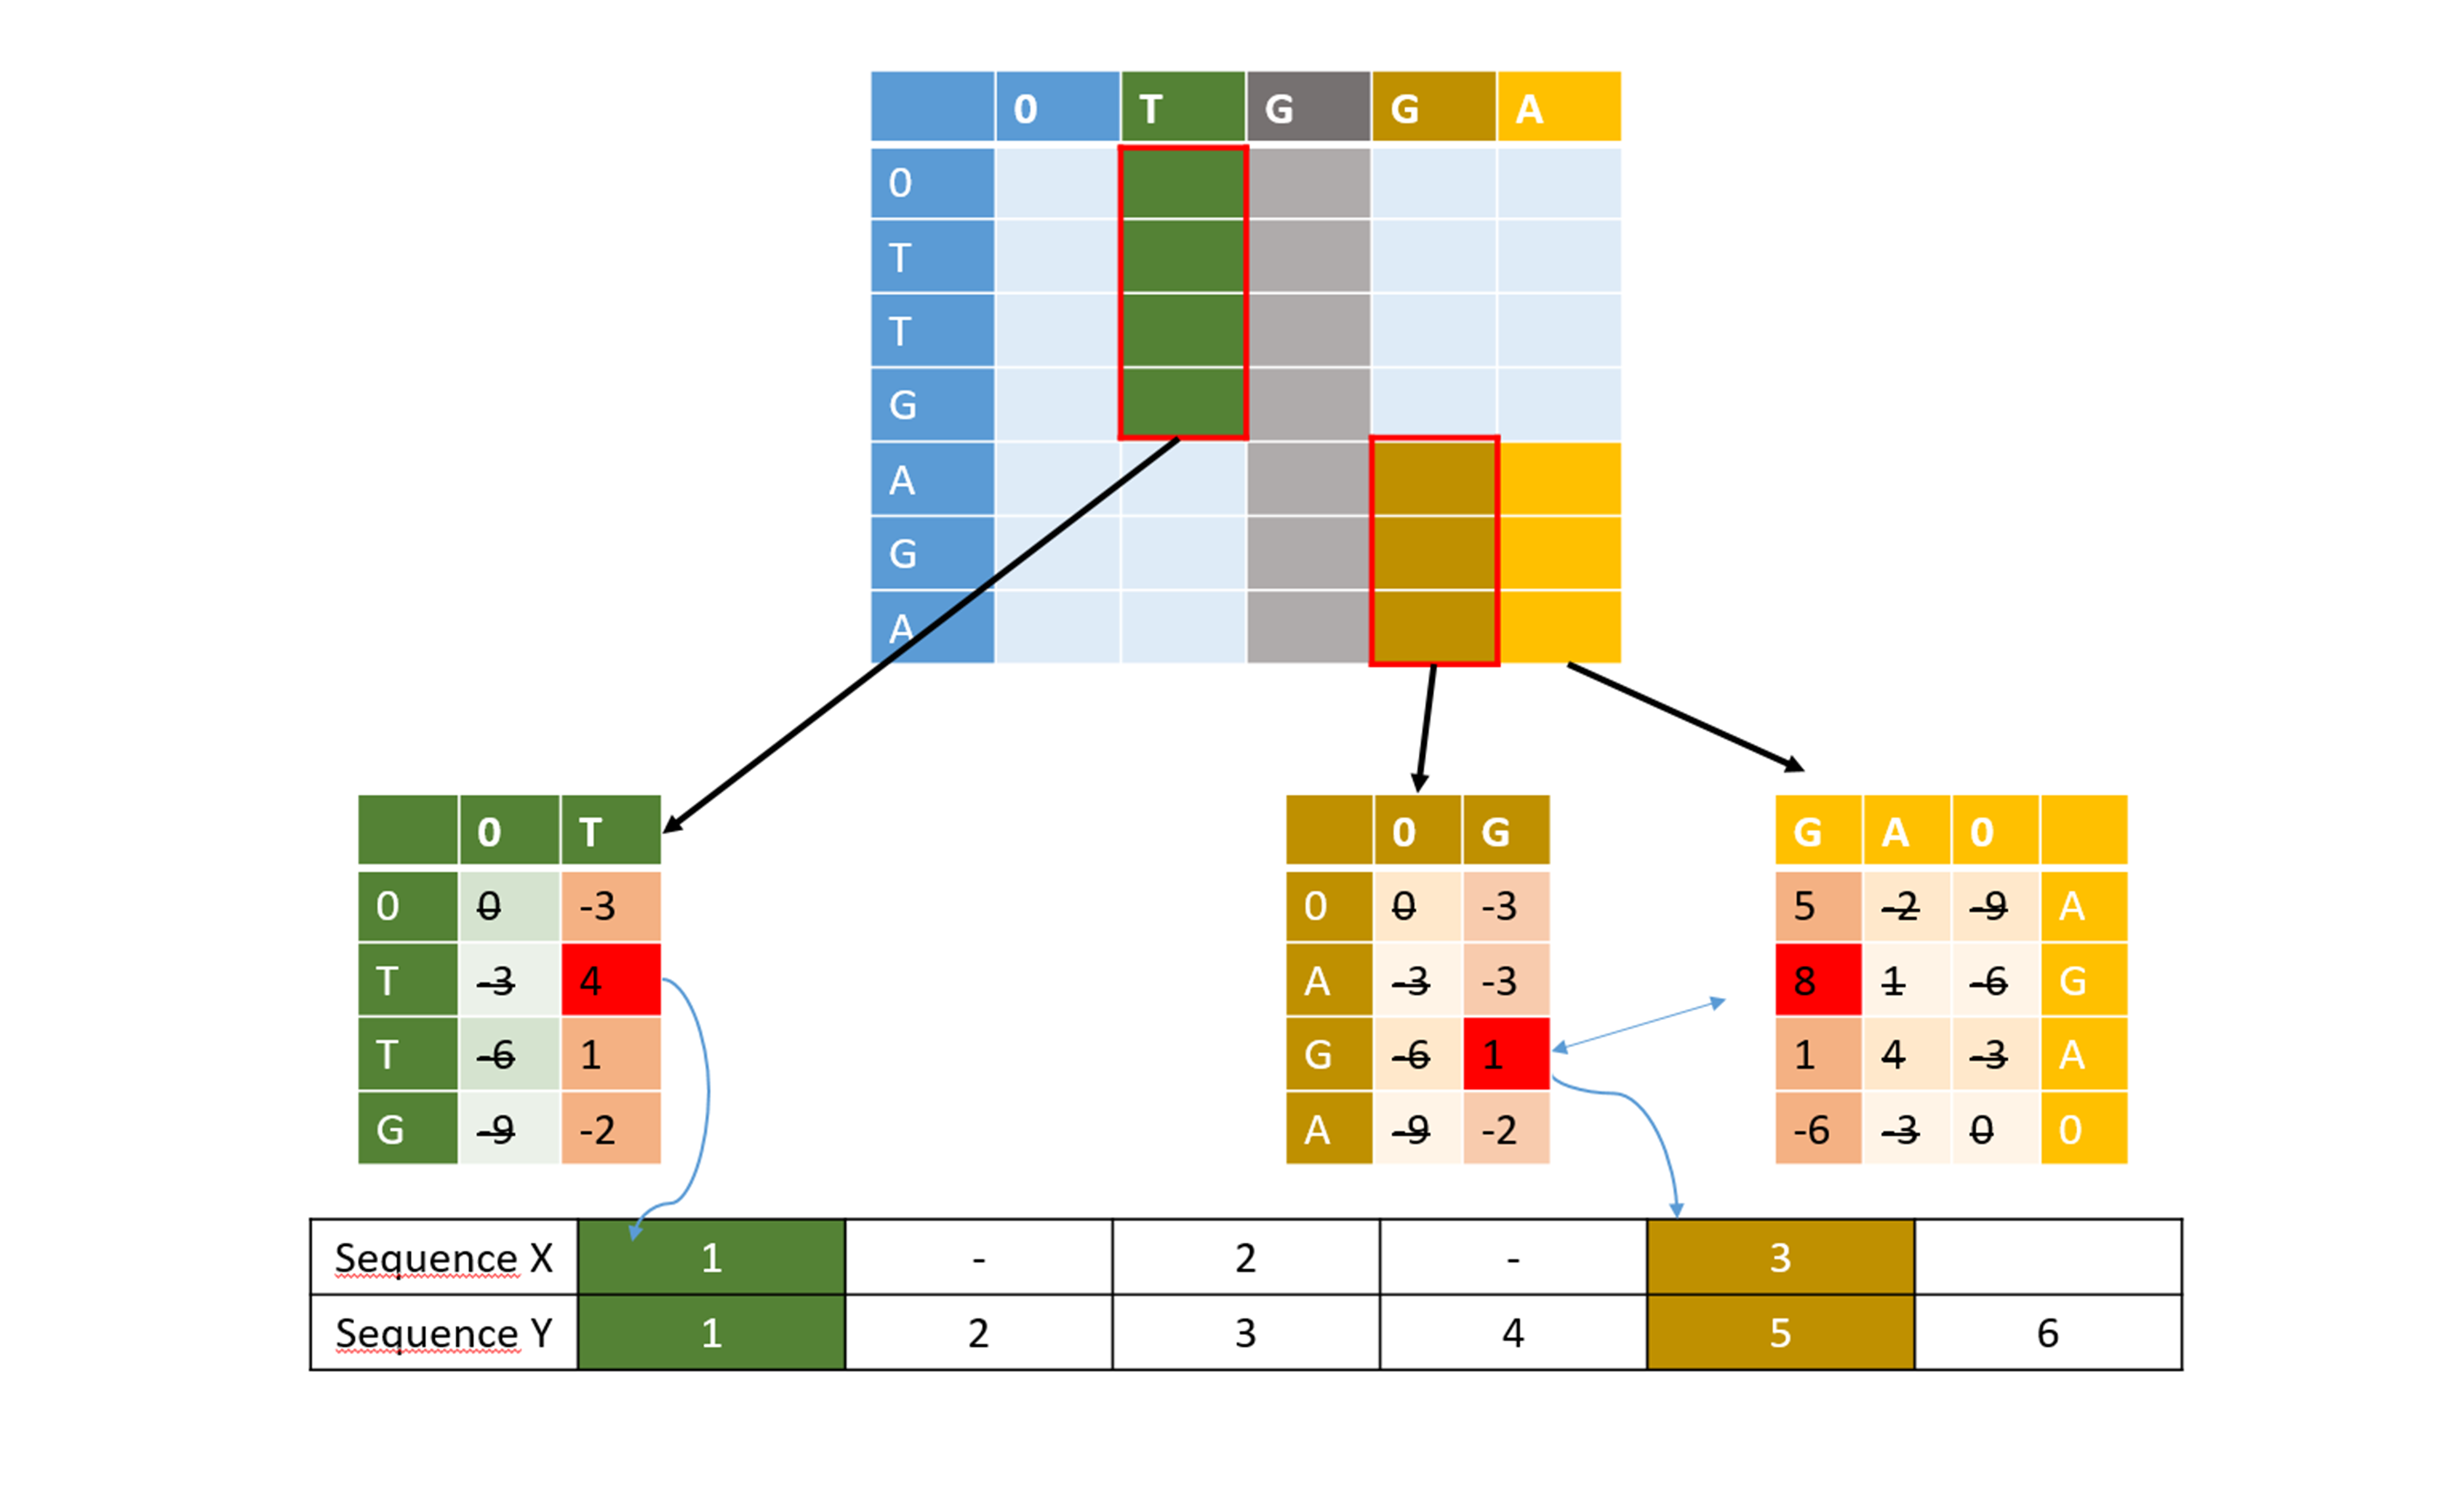
\includegraphics[scale=0.25]{img/Hirschberg_Step2.png}
   	\label{Step2}
   	\caption{Step 2 - calculating the needleman wunsch alignments for the sub sequences.}
  \end{figure}
  
  In step 3 the trivial case was now in the yellow area (\ref{Step3} -yellow arrea). And the last position for aligning was filled into the result matrix. 
 
  \begin{figure}[h]
    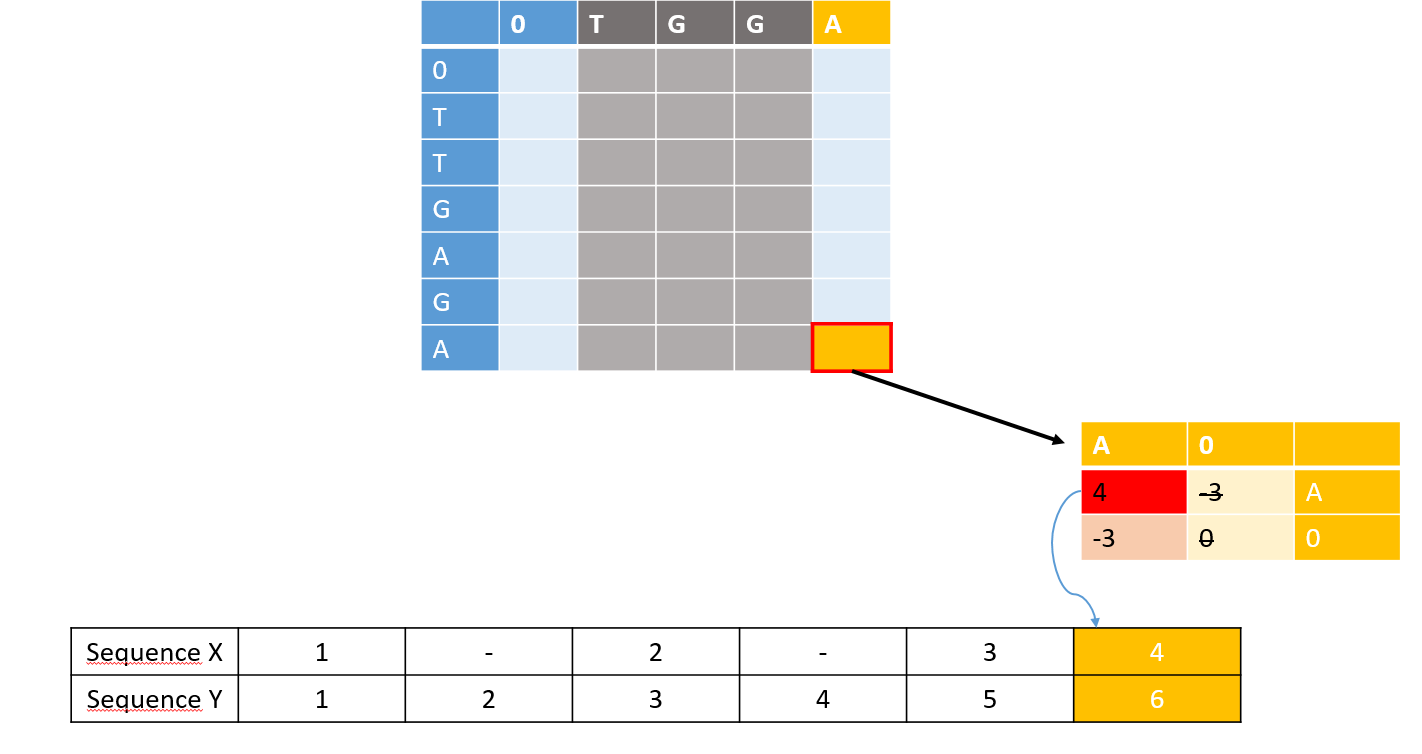
\includegraphics[scale=0.25]{img/Hirschberg_Step3.png}
	\label{Step3}
	\caption{step 3 - final trivial case}
  \end{figure}
    
    In step 4 the interpretation of the result array was processed. This means, that if a position was in the result array, both letters were aligned according to the postions. If there was no position in the array, a gap was filled in (\ref{Step4}).
    
  \begin{figure}[h]
   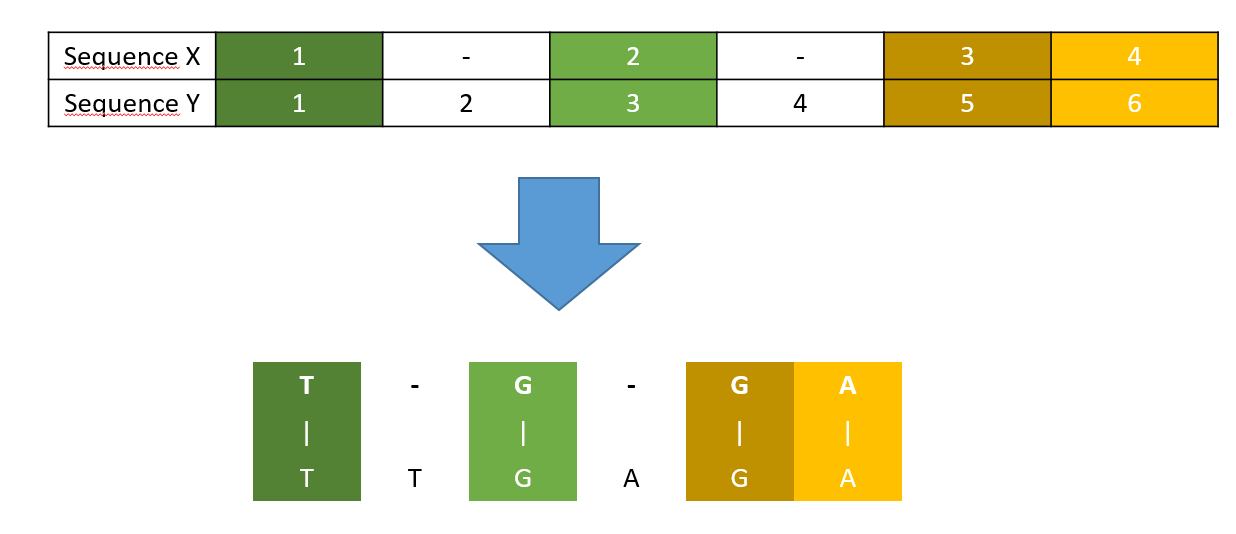
\includegraphics[scale=0.25]{img/Hirschberg_Step4.png}
   \label{Step4}
   \caption{Interpretation of the Result array.}
   \end{figure}
   
   
   
 \section*{Exercise 2 - \textsl{Do scoring matrices have expected score smaller than zero?}}
 
 The substitution matrices were evaluated according to the expectancy value formula given in the lecture, the substitution matrices were evaluated with the assumption of uniform distributed amino acids in two sequences.
 \begin{equation*}
 \sum_{a,b \in \Sigma}p_a p_b s(a,b)
 <=>  (\sum_{a,b \in \Sigma} s(a,b))  p_a p_b
 \label{expectance}
 \end{equation*}
 
 For the determination of one expectance value, $p_a$ and $p_b$ were each substituted with $1/20$, for the probabilistic occurrence in sequences with uniform distributed amino acids. The sum was calculated via R and the total summation of the substitution matrix \ref{expectance}.The result for each matrix can be seen in table \ref{Results-Expectance}.
 
 \begin{table}[h]
 \begin{tabular}{|c|c|}
 	\hline \rule[-2ex]{0pt}{5.5ex} Substitution Matrix & Expectance Value \\ 
 	\hline \rule[-2ex]{0pt}{5.5ex} BLSOUM50 & -1.155 \\ 
 	\hline \rule[-2ex]{0pt}{5.5ex} BLOSUM52 & -1.065 \\ 
 	\hline \rule[-2ex]{0pt}{5.5ex} BLOSUM80 & -2.3275 \\ 
 	\hline \rule[-2ex]{0pt}{5.5ex} PAM250 & -1.14 \\ 
 	\hline \rule[-2ex]{0pt}{5.5ex} PAMN & 0.155 \\ 
 	\hline 
 \end{tabular} 
 
   	\label{Results-Expectance}
   	\caption{Result of the calculation with each given substitution matrix according to equation}
 \end{table}
 
 As a conclusion we want to state, that all substitution matrices are possible feasible matrices. Except of the PAMN matrix, which has a positive expectancy value, which could lead to wrong conclusion.
One Aspect we also want to state, is that we did not calculate the values for the matrices with the unknown sign x or X. and the B or Z sign,  which stands for two amino acids. Although it would be possbile to use the unknown sign, if they are also uniform distributed in a sequence. But as a result of the wanted comparison, between matrices which didn't contain these signs, we did not use these columns and rows in our calculations.
 
 \section*{Exercise 3 - \textsl{Needleman-Wunsch algorithm for affine gap scores}}
 
  
\end{document}